%=================================================
\sectionDark{Random Forest}
%=================================================
\begin{frame}
  \frametitle{Introducci�n -- I}
  \only<1>{\alert{Hasta ahora:}\\ \qquad Un conjunto de entrenamiento $\rightarrow$ Un �rbol
  de clasificaci�n\\}

  \only<2>{\alert{Random forest:}\\ \qquad Un conjunto de entrenamiento $\rightarrow$ Varios �rboles
    de clasificaci�n\\}

  \vspace{0.3cm}

  \begin{columns}
    \begin{column}{0.5\textwidth}
      \begin{tabular}{ccccc}
        Sexo & Altura & Peso & Exp. & Act. \\ \hline
        H & 1,55 & 45 & A+ & F�tbol \\
        H & 1,67 & 58 & C & F�tbol \\
        M & 1,45 & 45 & B & F�tbol \\
        M & 1,58 & 50 & A+ & P�del \\
        H & 1,20 & 40 & B & F�tbol \\
        M & 1,80 & 60 & A & P�del \\
        $\cdots$ & $\cdots$ & $\cdots$ & $\cdots$ & $\cdots$ \\ \hline
      \end{tabular}
    \end{column}
    \begin{column}{0.5\textwidth}
      \vspace{0.3cm}
      \includegraphics<1>[width=\textwidth]{images/randomForest/1arbol.png}
      \includegraphics<2->[width=\textwidth]{images/randomForest/bosque.png}
    \end{column}
  \end{columns}

\end{frame}


\begin{frame}
  \frametitle{Introducci�n -- II}

  \begin{block}{Random forest\footnote{T�cnica propuesta por primera vez en \cite{randomForest}.} (\textcolor{red}{No me gusta este t�tulo})}
    \begin{itemize}
    \item �C�mo se clasifica una instancia?
    \item �C�mo se generan varios �rboles con el mismo conjunto de
      entrenamiento?
    \item �C�mo se genera un �rbol en concreto?
    \end{itemize}
  \end{block}

   
\end{frame}


\begin{frame}[fragile,fragile]
  \frametitle{Clasificaci�n de instancias}
  
  Al existir varios �rboles, pueden existir varias clases posibles para una
  instancia.\\
  \quad La clase final ser� aquella que m�s veces aparece elegida (\alert{moda}).
\begin{lstlisting}[frame=single, numbers=left]
clasifica(x):
  for_each a in arboles:
     cjto += clasifica(x, a)

  return moda(cjto)
\end{lstlisting}

\begin{columns}
  \begin{column}{0.6\textwidth}
    \flushright
    \includegraphics<1>[scale=0.2]{images/randomForest/arbol_class1.png}
    \includegraphics<2->[scale=0.2]{images/randomForest/arbol_class2.png}
  \end{column}
  \begin{column}{0.4\textwidth}
    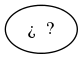
\includegraphics[scale=0.2]{images/randomForest/nodo.png}
  \end{column}
\end{columns}

\end{frame}


\begin{frame}
  \frametitle{Generaci�n de �rboles --- Selecci�n de instancias}
\end{frame}

\begin{frame}
  \frametitle{Generaci�n de �rboles --- Selecci�n de atributos}
\end{frame}



%
%
%%%
%%% Local Variables:
%%% mode: latex
%%% TeX-master: "PRESENTACION.tex"
%%% End:
